\begin{solution}{hard}
First, note that all voltometers are identical while the ammeters are not. Since the voltometers, are identitcal, it would be wise to see the internal resistance that they have as it will most likely help to solve the problem. We are given the reading of the first ammeter to be $I_1 = 2.9\;\mathrm{mA}$ and the reading of the second ammeter to be $I_2 = 2.6\;\mathrm{mA}$. Therefore, the current drop is $\Delta I = 0.3\;\mathrm{mA}$. By fact 3 (Ohm's Law), we write:
\[r = V/\Delta I \implies r = 3\times 10^4\;\mathrm{\Omega}.\]Note that there is an extra factor of $10^{2}\;\mathrm{\Omega}$ since the current is measured in milliamperes. Now, by idea 8, we know that it is sometimes convenient to consider the Kirchoff’s current law for a whole region and not just for a single circuit node: the sum of currents entering the region equals to the sum of outgoing currents. In this case, we will consider the region marked by the circle below:

\begin{center}
    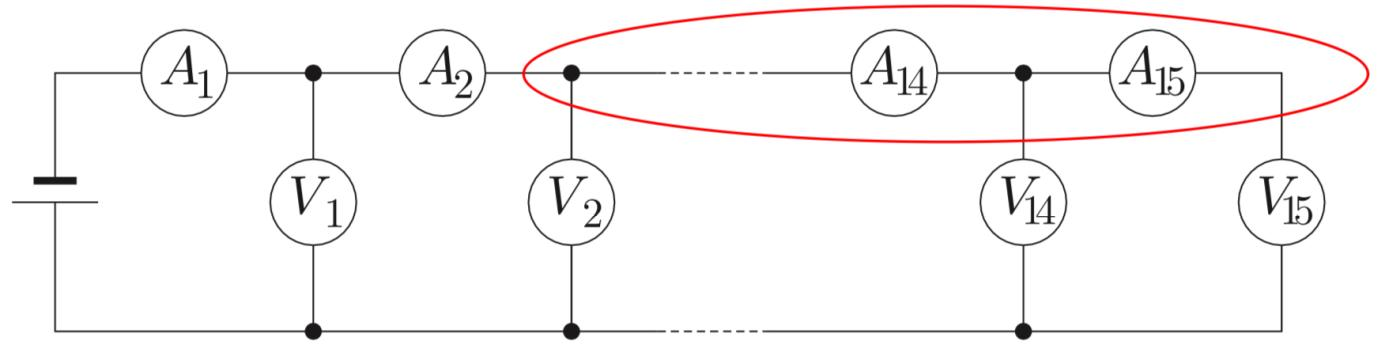
\includegraphics[width=0.6\linewidth]{Figures/7_sol.jpg}
\end{center}

The total voltage of the region will then be given by
\[V_{\text{region}} = \sum_{i = 2}^{15} V_i = \sum_{i = 2}^{15} r (I_i - I_{i  +1}) = r\sum_{i = 2}^{15} (I_i - I_{i  +1})\]where $i = 2, 3, \dots, 15$ represents a node in the circuit. The total voltage will then be given as
\begin{align*}
V_{\text{region}} &= r\sum_{i = 2}^{15} (I_i - I_{i  +1})\\
&= r(I_2-I_3) + \dots + r(I_{14}-I_{15}) + rI_{15}  \\
&= rI_2 \\
& = \boxed{78\;\mathrm{V}}.
\end{align*}
\end{solution}